%% 2 ::: Desenvolvimento
\chapter{Desenvolvimento}
%% Interlúdio do [Desenvolvimento] %%
    ...
%% Fim do Interlúdio do [Desenvolvimento] %%


%% 2 ::: Desenvolvimento
%% 2.1
\section{Metodologia de Pesquisa}
%% Interlúdio do [Metodologia de Pesquisa] %%
Para os testes deste trabalho estão sendo usados os mesmo problemas utilizados por \cite{Kacem2002}, e já são largamente usados na literatura. Sendo representados por $[j, o, m]$ em que $j$ é a quantidade de \textit{jobs}, $o$ é a quantidade de operações e $m$ a quantidade de máquinas. Para observar o comportamento do algoritmo em diversos cenários foram escolhidos problemas de tamanhos variados, sendo eles $[4, 12, 5]$, $[10, 29, 7]$, $[10, 30, 10]$ e $[15, 56, 10]$. Os problemas de teste podem ser encontrados nos apêndices do trabalho.\\
%
\indent Os algoritmos foram executados no ambiente de nuvem Google Colab Code sendo executado no motor \textit{Python 3 Google Compute Engine Backend}. Para a execução foi utilizado um \textit{runtime} com processadores comuns (CPU) e 12 Gigabytes de memória RAM.\\
%
%
\indent Para que possibilitar uma análise de dados mais detalhada e a geração de gráficos para representação nesse trabalho, foram implementados no código pontos de salvamento de dados, para salvar em formato de binários do NumPy, utilizando a função \code{np.savedata}, as informações de execuções e de datasets.\\
\indent Dentre esses dados estão o espaço de soluções gerado, a quantidade de rodadas feitas, o histórico da variável $gBest$, o número de mudanças de $pBest$, o histórico de posição das partículas e as soluções finais encontradas.
%% Fim do Interlúdio do [Metodologia de Pesquisa] %%

%% 2 ::: Desenvolvimento
%% 2.1 ::: Metodologia de Pesquisa
%% 2.1.1

%% 2 ::: Desenvolvimento
%% 2.2
\section{Arquitetura}
%% Interlúdio do [Arquitetura] %%
A arquitetura de um projeto de é um fator que impacta diretamente no seu desempenho, porém como o objetivo desse trabalho é entender como o algoritmo PSO se comporta diante das alterações propostas, foi necessário o desenvolvimento de uma arquitetura que represente o problema de maneira mais abstrata.
%% Fim do Interlúdio do [Arquitetura] %%

%% 2 ::: Desenvolvimento
%% 2.2 ::: Arquitetura
%% 2.2.1
\subsection{Design do Projeto}
Por esse trabalho ser desenvolvimento dentro de um grupo de estudos, foi optado por usar uma estrutura de projeto mais didática e de fácil entendimento, de maneira que possa ser facilmente reutilizada por futuros estudantes. Porém, essa escolha acarreta uma certa perda de desempenho, porém, como se trata de um trabalho que visa explorar como cada tipo de alteração impacta o algoritmo, essa perca de desempenho não se torna um defeito.\\
\indent O projeto foi desenvolvido na linguagem de programação Python versão 3.9.7 e utiliza além das bibliotecas básicas da linguagem, as bibliotecas:
\begin{itemize}
    \item NumPy (versão 1.21.3)
    \item MatPlotlib (versão 3.4.3)
\end{itemize}

\noindent O MatPlotlib foi utilizado para a geração de: 
\begin{itemize}
    \item Gráficos de Dispersão (\textit{Scatter Plot}) para representar a posição das partículas da população.
    \item Gráficos de Superfície (\textit{Surface Plot}) para representar o espaço de soluções.
    \item Gráficos de Barra Horizontal (\textit{Horizontal Bar Plot}) para representar um diagrama de Gantt com a solução do agendamento.
\end{itemize}

\noindent O NumPy foi utilizado para: 
\begin{itemize}
    \item Grandes arranjos multi dimensionais de dados. 
    \item Funções randômicas de escolha.
    \item Ordenação de dados.
    \item Operações de cálculo como raiz quadrada e potenciação.
    \item Funções de escolha de valores máximos e mínimos.
    \item Modelagem, união e remodelagem de matrizes.
    \item Representações e calculo de vetores de movimentação.
\end{itemize}
        
Para trazer mais clareza ao código foi optado por criar algumas classes para a representação de entidades e abstração de lógicas. Dentre elas estão:
\begin{itemize}
    \item Classe de Partícula, que faz a representação de uma entidade de partícula e armazena sua posição, velocidade e direção. Faz a inicialização da partícula com valores aleatórios de posição, velocidade e direção. E estabelece métodos para calcular o movimento da partícula e o valor da qualidade de sua nova posição.

    \item Classe de \textit{encoding}, responsável por ler e interpretar os arquivos de instância de um problema, criar uma representação para de solução, e então gerar o espaço de soluções com soluções geradas aleatoriamente.

    \item Classe de \textit{decoding}, responsável por decodificar uma solução no padrão de representação estabelecido pela classe de \textit{encoding} e calcular o \textit{fitness} dessa solução. Essa classe também estabelece o método que gera o gráfico de Gantt para representar visualmente a solução.
\end{itemize}

\indent Como o PSO é um algoritmo estocástico, ou seja, seu resultado é fruto de eventos não previsíveis foi decidido que para obter uma média real dos desempenhos de cada algoritmo, em cada uma das 30 execuções será gerado um novo espaço de soluções e uma população inicial diferente.\\
\indent E em cada uma dessas execuções será passado para cada um dos algoritmos uma \textit{deepcopy} do espaço de soluções e da população inicial, para que os diferentes algoritmos trabalhem com base nos mesmos dados iniciais, para assim tem uma análise mais justa.\\
\indent Para que a análise dos dados possa ser feita mais detalhadamente, foram implementados alguns pontos de salvamento de dados, para salvar em arquivo texto as representações da população e do espaço de soluções gerados aleatoriamente, assim como a quantidade de rodadas feitas, o histórico da variável $gBest$, o número de mudanças de $pBest$, o histórico de posição das partículas e as soluções finais encontradas.
%
Na \hyperref[fig:fluxo-design]{Figura \ref{fig:fluxo-design}} é possível ver uma representação das relações e fluxo de dados entre as classes.

%
\begin{figure}[ht]
    \centering
    \caption{Fluxo de dados}
    \label{fig:fluxo-design}
    %\includegraphics[width=\textwidth]{}
\end{figure}

%
%% Fim do [Design do Projeto] %%
    

%% 2 ::: Desenvolvimento
%% 2.2 ::: Arquitetura
%% 2.2.2
\subsection{Espaço de Soluções}
%% Interlúdio %%
O espaço de soluções (também chamado espaço de busca) é um conceito que define um espaço imaginário aonde cada ponto desse espaço é uma possível solução para o problema em questão. 
Um espaço de soluções pode ser representado de diversas maneiras, como listas e grafos, mas em problemas de optimização normalmente se usa uma representação na forma de uma matriz.\\
%% Fim do [Interlúdio] %%
%% 2 ::: Desenvolvimento
%% 2.2 ::: Arquitetura
%% 2.2.2 ::: Espaço de Soluções
%% 2.2.2.1
%\subsubsection{Representações}
\indent Nessa representação em forma de matriz cada localização $[i, j]$ tem uma solução valida para o problema, e o algoritmo em questão tem a tarefa de encontrar qual dessas posições tem a melhor solução, ou uma solução boa o suficiente. Na 
\hyperref[fig:solution-space]{Figura \ref{fig:solution-space}} 
é mostrado uma representação conceitual de um espaço de soluções em forma de matriz.\hfill
            
\begin{figure}[ht]
    \centering
    \caption{Representação de uma matriz de espaço de soluções}
    \label{fig:solution-space}
    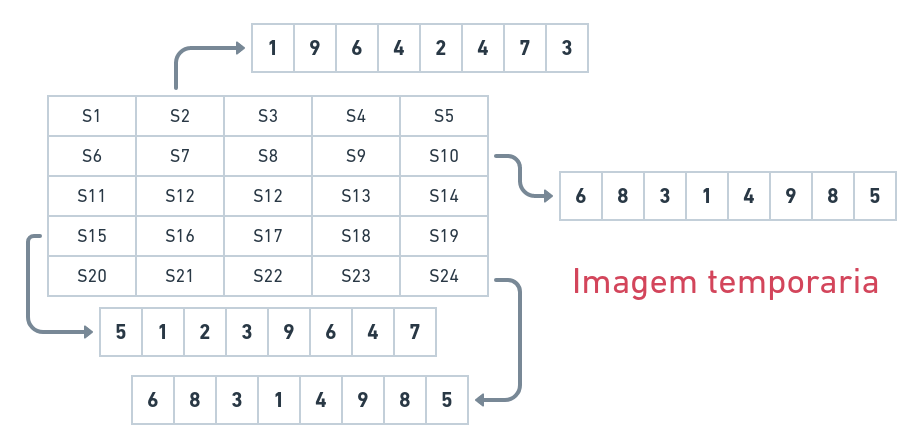
\includegraphics[width=\textwidth]{assets/solution.png}
    %\small{Incluir a imagem do exemplo de espaço de solução aqui}
\end{figure}

Algumas das implementações encontradas em bibliotecas de algoritmos populacionais de código aberto como \textit{PySwarms} utilizam internamente um sistema de representação de espaço de soluções de uma única dimensão, ou seja, uma lista simples, e utiliza uma função para transformar uma posição $[x,y]$ em um índice da lista. Essa implementação provavelmente foi escolhida por ser na maioria dos casos, mais rápida em comparação a uma abordagem de duas dimensões.\\
%% Fim do [Representações] %%
%% 2 ::: Desenvolvimento
%% 2.2 ::: Arquitetura
%% 2.2.2 ::: Espaço de Soluções
%% 2.2.2.2
%\subsubsection{Gráficos de análise}
\indent Como esse trabalho tem como foco uma exploração e implementação mais didática foi optado a utilização de uma representação em forma de uma matriz com duas dimensões, utilizando a biblioteca \textit{NumPy}. Essa abordagem em matriz de duas dimensões também facilita a geração de gráficos para representação visual, como, por exemplo, passar a matriz de soluções pela função de avaliação e assim obter um valor de \textit{fitness} para cada ponto do espaço de soluções, como é possível ver na 
\hyperref[fig:surfaceplot]{Figura \ref{fig:surfaceplot}} 
na qual os valores mais acima e mais escuros tem um valor de \textit{fitness} mais alto (ou seja, pior), e os valores mais abaixo e mais claros tem um \textit{fitness} mais baixo (ou seja, melhor).

\begin{figure}[ht]
    \centering
    \caption{Gráfico de Superfície representando um espaço de soluções}
    \label{fig:surfaceplot}
    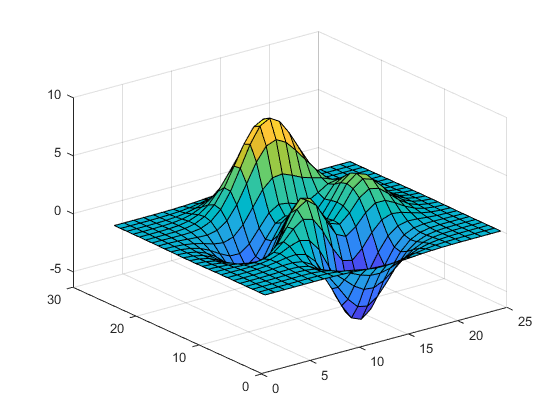
\includegraphics[width=\textwidth]{assets/surfaceplot.png}
\end{figure}

Esses gráficos se mostraram uteis ao decorrer do desenvolvimento deste trabalho, servindo para validar detectar erros na função de inicialização do espaço de soluções.\\
%% Fim do [Gráficos de Analise] %%
%% 2 ::: Desenvolvimento
%% 2.2 ::: Arquitetura
%% 2.2.2 ::: Espaço de Soluções
%% 2.2.2.3
%\subsubsection{Influencia na Solução}
\indent A geração do espaço de soluções é muito importante para algoritmos como o PSO 
que funciona com base na movimentação conforme as médias de melhores posições, 
devido a isso, o PSO tente a ter problemas com convergência prematura em mínimos locais.\\
\indent Os mínimos locais são fenômenos onde dentro de uma parte do espaço de soluções existe um ponto que é melhor que a média dos pontos a sua volta, porém não é o melhor entre o todo o espaço de soluções, como é possível ver na \hyperref[fig:ex-minimolocal]{Figura \ref{fig:ex-minimolocal}}.\newline
\begin{figure}[ht]
    \centering
    \caption{Exemplo de um mínimo local}
    \label{fig:ex-minimolocal}
    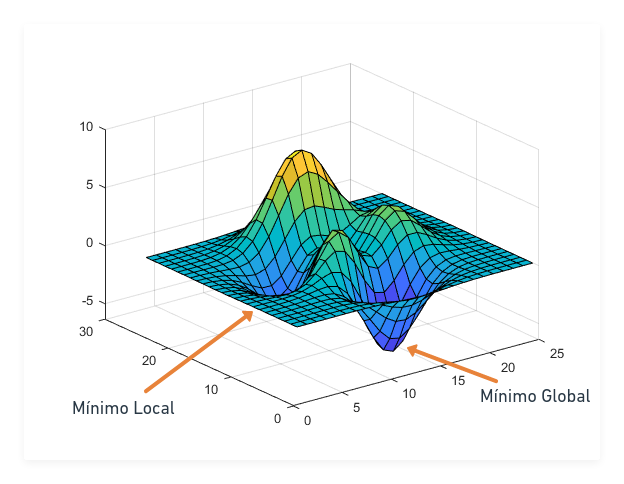
\includegraphics[width=\textwidth]{assets/minimo_local.png}
    %\small{}
\end{figure}
Por esse ponto se destacar entre seus vizinhos o algoritmo pode ficar preso nesta região, pois a média local sempre tende para o ponto onde está o mínimo local.\\
Como o PSO se baseia na média local e global, se houver mais de um mínimo local e quantidades equivalentes de partículas da população forem distribuídas para esses pontos, as partículas podem ficar presas já que as forças se balanceiam e o $gBest$ não muda mais.\\
%
\indent Já a convergência prematura acontece quando a um mínimo local e por coincidência a posição inicial da maioria das partículas da população tende a ser atraído para o mínimo local, logo a maioria da população para nesse ponto e o algoritmo termina antes de encontrar uma solução tão boa quando seria possível.\\
%% Fim do [Influencia na Solução] %%
%% 2 ::: Desenvolvimento
%% 2.2 ::: Arquitetura
%% 2.2.2 ::: Espaço de Soluções
%% 2.2.2.4
%\subsubsection{Implementação}
\indent Durante a implementação de um algoritmo para geração do espaço de soluções, foram percebidos diversos detalhes que influenciam fortemente na qualidade final do algoritmo. Nessa seção será analisado alguns desses pontos.\\
%\subsubsubsection{Inicialização}
\indent Um ponto importante percebido na implementação é como sera inicializado o \textit{array} onde será armazenado o espaço de soluções.\\
\indent O NumPy disponibiliza trés métodos de inicialização para um novo \textit{array} sem um valor de preenchimento, dos quais cada um demonstrou um problema diferente para a implementação. Dentre eles: 
\begin{itemize}
    \item \textit{numpy.zeros}: Ao inicializar o \textit{array} com todos os valores preenchidos com o valor "$0$", devido ao processo de embaralhamento das operações, o algoritmo pode acabar gerando resultados errôneos. Por não existir uma maquina $M_0$ algumas operações não eram consideradas no resultado, e devido à falta de algumas operações, a solução em questão tinha um valor de \textit{fitness} menor, o que tendia a fazer essa solução errônea a melhor.

    \item \textit{numpy.ones}: Ao inicializar o \textit{array} com todos os valores preenchidos com o valor "$1$", o algoritmo gerava soluções que tendiam a sobre carregar a máquina $M_1$ e assim os resultados finais tendiam a ter um valor de \textit{fitness} mais alto.

    \item \textit{numpy.empty}: Esse método de inicialização diferentemente dos outros, não defini nenhum valor para os registros da matriz, somente aloca um bloco de memória (semelhante ao \textit{malloc} da linguagem C), o que o torna mais rápido, porém ele traz o revés de possivelmente ter valores errados, pois por simplesmente alocar um bloco de memória, o \textit{array} pode ser inicializado com valores estranhos devido a lixo de memória.
\end{itemize}

\noindent Devido aos problemas citados acima, acaba sendo necessário de qualquer maneira percorrer todo o \textit{array} para setar valores. \newline 
Então foi optado por utilizar um método de preenchimento de valores aleatório, 
gerados pela função \textit{numpy.random.choice} que gera um \textit{array} de valores aleatórios seguindo uma distribuição uniforme, 
conforme demonstrado no Gráfico da \hyperref[fig:distrib-uniforme]{Figura \ref{fig:distrib-uniforme}}.

\begin{figure}[ht]
    \centering
    \caption{Gráfico de distribuição de valores gerados pela função aleatória}
    \label{fig:distrib-uniforme}
    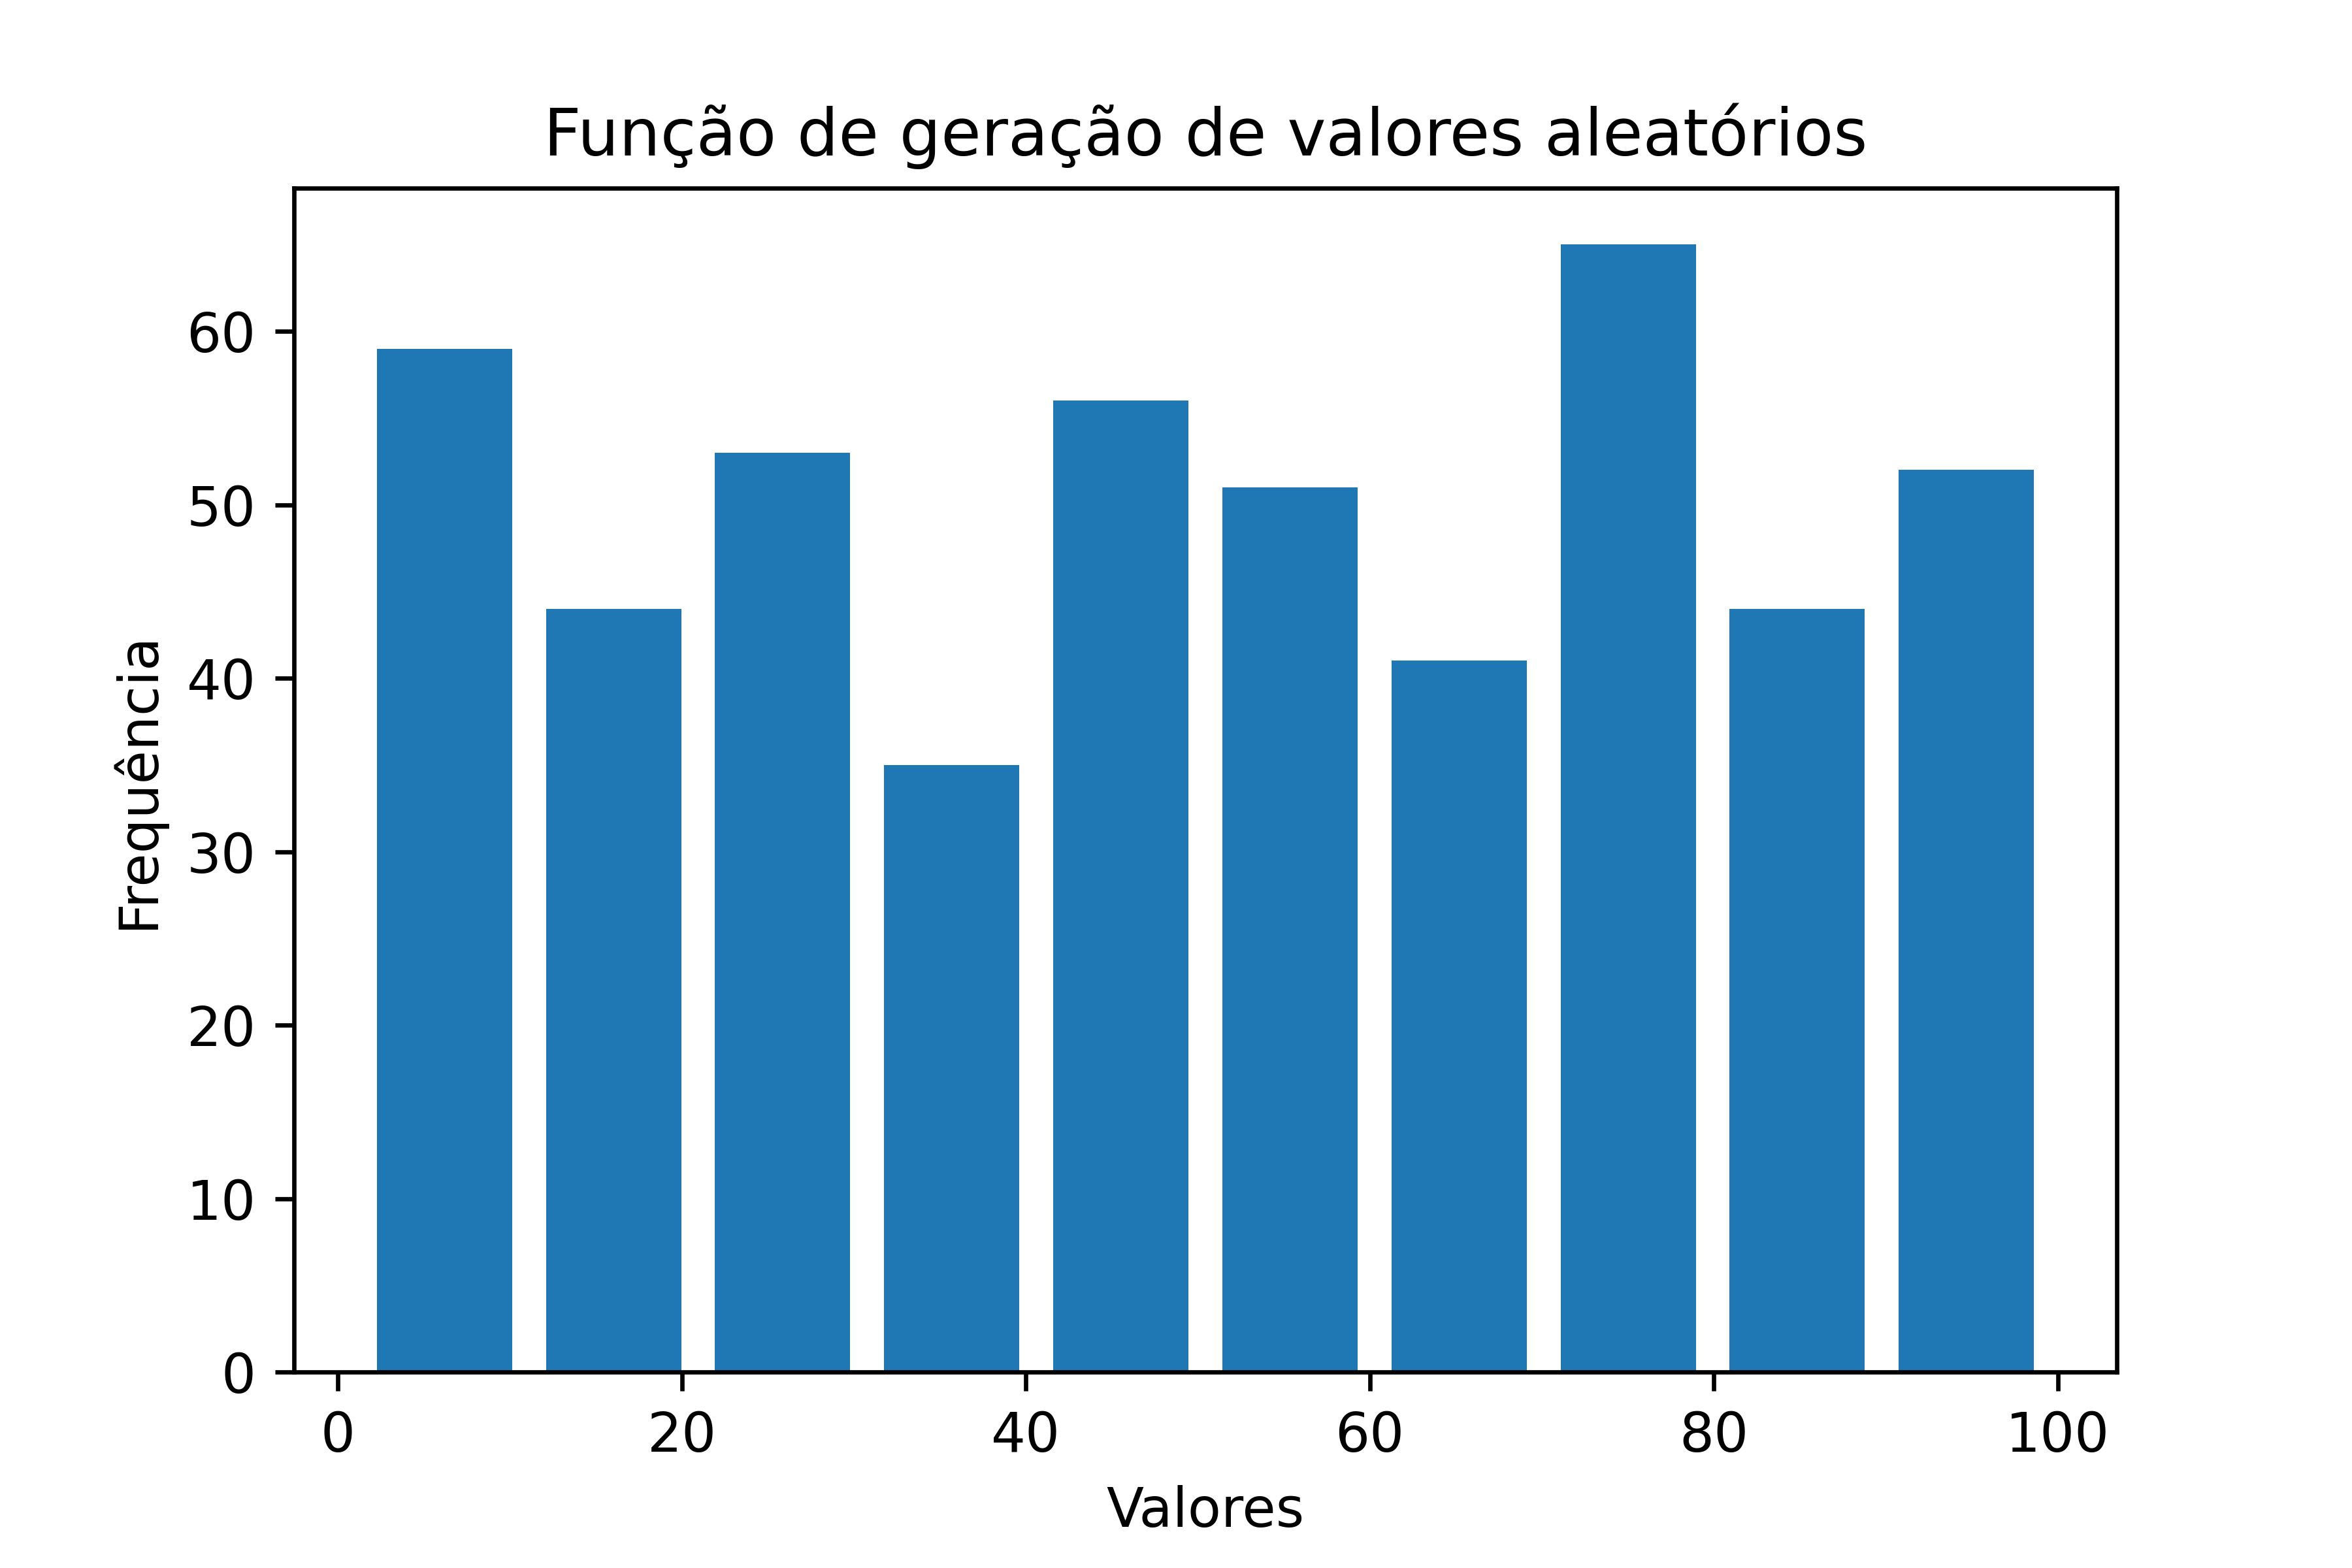
\includegraphics[width=\textwidth]{assets/hist_uniform.png}
\end{figure}

%
%% Inicialização do Array

Após as análises citadas acima foi feito uma modelagem e desenvolvido para esse trabalho o algoritmo de inicialização do espaço de soluções representado pelo 
\hyperref[alg:generate-solution-space]{Pseudocódigo \ref{alg:generate-solution-space}}.
Além disso, a implementação real em Python está no apêndice x desse trabalho.\\
%% Todo - Apêndice
%%%%%%%%%%%%%%%%%%%%%%%%%%%%%
\begin{algorithm}
\caption{Pseudocódigo de geração do espaço de soluções}\label{alg:generate-solution-space}
\begin{algorithmic}
\State espaço soluções $\gets$ lista vazia
\State contador  $\gets$ 0
\While{ contador $\leq$ tamanho espaço de soluções}
  \State solução $\gets$ lista vazia
  \State embaralhar(operações)
  \State embaralhar(jobs)
  \State embaralhar(maquinas)
  \State solução[operações] $\gets$ remover ultimo elemento(operações)
  \State solução[jobs] $\gets$ remover ultimo elemento(jobs)
  \State solução[maquinas] $\gets$ remover ultimo elemento(maquinas)
  \State espaço soluções $\gets$ adicionar(solução)
\EndWhile
\end{algorithmic}
\end{algorithm}
%%%%%%%%%%%%%%%%%%%%%%%%%%%%%
%% Fim do [Implementação] %%
%% Fim do [Espaço de Soluções] %%
%% 2 ::: Desenvolvimento
%% 2.2 ::: Arquitetura
%% 2.2.3
\subsection{Partícula}
%% Interlúdio %%
Por se tratar de um algoritmo populacional focado em partículas, por isso o nome \textit{Particle Swarm Optimization} que significa Otimização por Enxame de Partículas, a representação dessa entidade, assim como sua geração, controle e movimentação, se mostra um dos principais pilares do algoritmo. Devido a critérios de legibilidade e facilitação de futuros estudos nesse trabalho foi optado por criar uma estrutura de classe bem definida para essa representação e controle.
%% Fim do [Interlúdio] %%
%% 2 ::: Desenvolvimento
%% 2.2 ::: Arquitetura
%% 2.2.3 ::: Partícula
%% 2.2.3.1
%\subsubsection{Implementação}
Nessa classe são guardados os valores de: posição, velocidade e $pBest$, além de outros dados utilizados para facilitar o gerenciamento como: valor da solução da sua atual posição, assim como seu valor de \textit{fitness} e o tamanho do espaço de soluções.\\
\indent Para fazer uma melhor movimentação foi optado por não usar uma variável de direção, mas sim uma variável que guarda a última posição onde a partícula esteve.\\
Além da armazenagem dos valores da partícula, a classe da Partícula também implementa algumas funções como:
%%
Função \textbf{\textit{fill\_with\_random\_values}} que gera uma posição inicial e uma velocidade aleatória para a partícula.\\
%%
Função \textbf{\textit{evaluate\_value}} que faz o cálculo do valor de \textit{fitness} da atual posição e a comparação do valor com o atual valor de $pBest$ e atualiza o $pBest$ caso o novo valor seja melhor.\\
%%
Função \textbf{\textit{update\_position}} que faz a movimentação da partícula.\\
\noindent A implementação de toda a classe de partícula está disponível no 
\hyperref[apd:particule-class]{Apêndice \ref{apd:particule-class}}
desse trabalho.\\
%
\indent Em implementações de código aberto como a já citada \textit{PySwarms}, também se utiliza uma representação de classe, porém sem nenhuma responsabilidade de cálculo de \textit{fitness}, atualização de posição ou de preenchimento de valores aleatórios na partícula.\\
%
%% Fim do [Representações] %%
%% 2 ::: Desenvolvimento
%% 2.2 ::: Arquitetura
%% 2.2.3 ::: Partícula
%% 2.2.3.3
%\subsubsection{Movimentação}
\indent A movimentação da partícula no espaço de soluções é o ponto mais importante dessa entidade. Pois, se não for feita da maneira certa pode fazer o algoritmo não desempenhar tão quanto o possível.\\
\indent Como a implementação do espaço de soluções foi feita utilizando uma representação matricial, o mecanismo de movimentação mais intuitivo seria uma movimentação por soma de inteiros.\\
\indent Aonde se tem uma direção e com base nessa direção se soma ou subtrai o valor de velocidade do eixo de movimento e assim se obtém uma nova posição, como mostrado no \hyperref[alg:int-sum]{Pseudocódigo \ref{alg:int-sum}}.
\begin{algorithm}
    \caption{Pseudocódigo de movimentação por soma de inteiros}\label{alg:int-sum}
\begin{algorithmic}
\If{direcao = CIMA}
  \State posicaoY = posicaoY + 1
\ElsIf{direcao = ESQUERDA}
  \State posicaoX = posicaoX - 1
\ElsIf{direcao = DIREITA}
  \State posicaoX = posicaoX + 1
\ElsIf{direcao = BAIXO}
  \State posicaoY = posicaoY - 1
\ElsIf{direcao = SUPERIOR ESQUERDA}
  \State posicaoX = posicaoX - 1
  \State posicaoY = posicaoY + 1
\ElsIf{direcao = SUPERIOR DIREITA}
  \State posicaoX = posicaoX + 1
  \State posicaoY = posicaoY + 1
\ElsIf{direcao = INFERIOR ESQUERDA}
  \State posicaoX = posicaoX - 1
  \State posicaoY = posicaoY - 1
\ElsIf{direcao = INFERIOR DIREITA}
  \State posicaoX = posicaoX + 1
  \State posicaoY = posicaoY - 1
\EndIf    

\end{algorithmic}
\end{algorithm}

Ou seja, tendo uma posição $[15, 7]$ sendo $15$ o valor de $x$ e $7$ o valor de $y$,
uma velocidade $2$ e a direção do movimento ser \textit{CIMA}, a nova posição é obtida incrementado a velocidade ao valor de $y$ da posição, ou seja $[15, 7+2]$, então a nova posição seria $[15, 9]$.\\
%
Essa abordagem funciona bem para uma movimentação simples em espaços 2D. Sendo inclusive muito utilizada no desenvolvimento de jogos com mapas baseados em ladrilhos (\textit{Tile-based} / \textit{Grid-based}).\\
\indent Porém, no caso do algoritmo PSO é necessário que ao calcular a nova posição, se considere a inércia e uma média entre o $pBest$ e o $gBest$, o que gera muitas vezes uma movimentação em ângulos mais específicos o que torna a abordagem de soma de inteiros muito complexa e limitada para esse cenário.\\
%%%%
\indent Então nesse trabalho foi desenvolvido um método de movimentação baseado em cálculos vetoriais que elimina esses problemas de movimentação além de facilitar a implementação de novos pontos de comparação (além do $pBest$ e $gBest$) para o cálculo da nova posição.\\
%\subsubsubsection{Movimentação Vetorial}
\indent Essa abordagem de movimentação é baseado no conceito de \textit{Produto Escalar} definido pela Álgebra Linear, e representa o produto interno padrão do espaço euclidiano sendo definido como uma operação binaria entre dois vetores.\\
\noindent Em um cenário aonde a posição da partícula é $position=[12,8]$ e $pBest=[10, 15]$, $gBest=[16,20]$ e $velocidade=[2,4]$.\\
\noindent Para encontrar a nova posição de uma partícula são utilizados:
\begin{itemize}
\item $\vec p$ Que representa o vetor entre a partícula e o $pBest$ 
(\hyperref[fig:vetor-p]{Figura \ref{fig:vetor-p}}).
\item $\vec g$ Que representa o vetor entre a partícula e o $gBest$ 
(\hyperref[fig:vetor-g]{Figura \ref{fig:vetor-g}}).
\item $\vec r$ Que representa o vetor final de movimento
(\hyperref[fig:vetor-r]{Figura \ref{fig:vetor-r}}).
\end{itemize}

\begin{figure}[!htb]
\begin{minipage}{\textwidth}

% 1º linha
\begin{minipage}{0.48\textwidth}
\centering
\caption{Vetor $\vec v$ de movimento}
\label{fig:vetor-v}
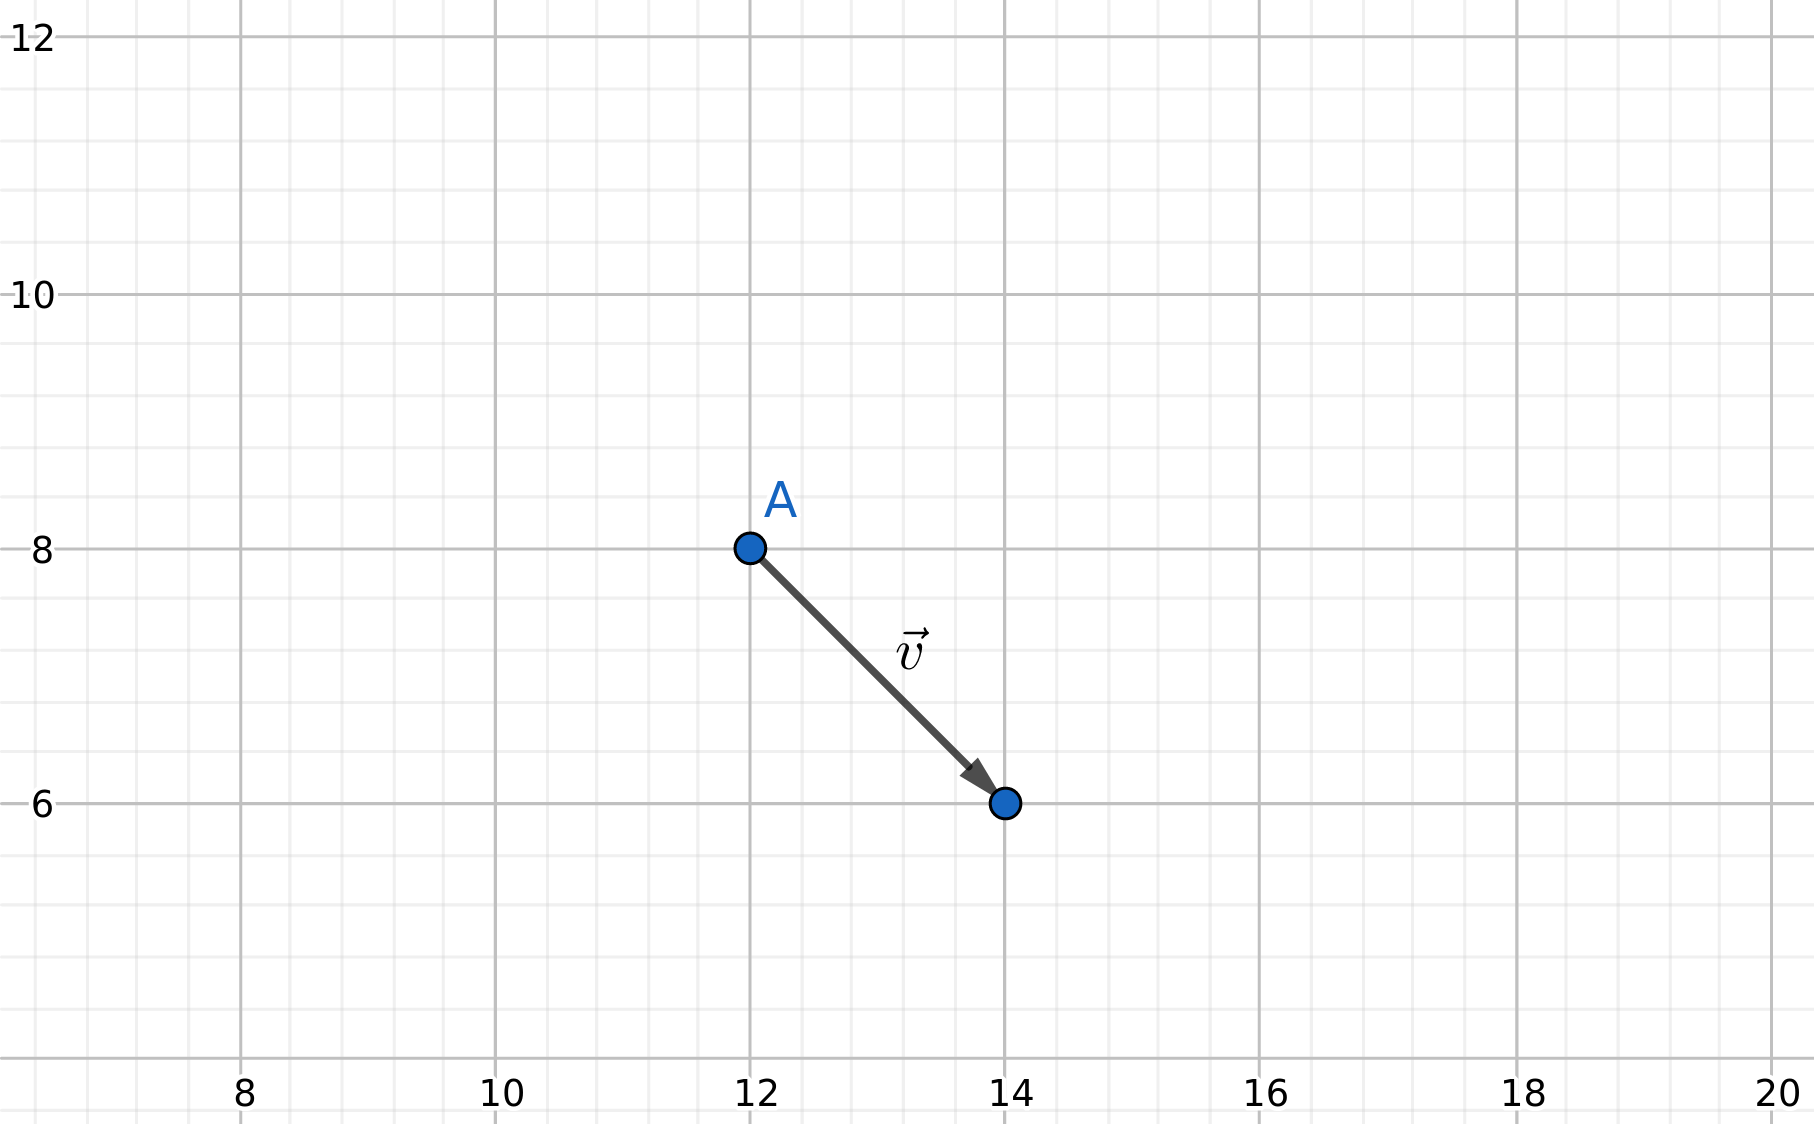
\includegraphics[width=.9\linewidth]{assets/vec1.png}
%\small{Incluir vetor v aqui}
\end{minipage}
\begin{minipage}{0.48\textwidth}
\centering
\caption{Vetor $\vec p$ de o $pBest$}
\label{fig:vetor-p}
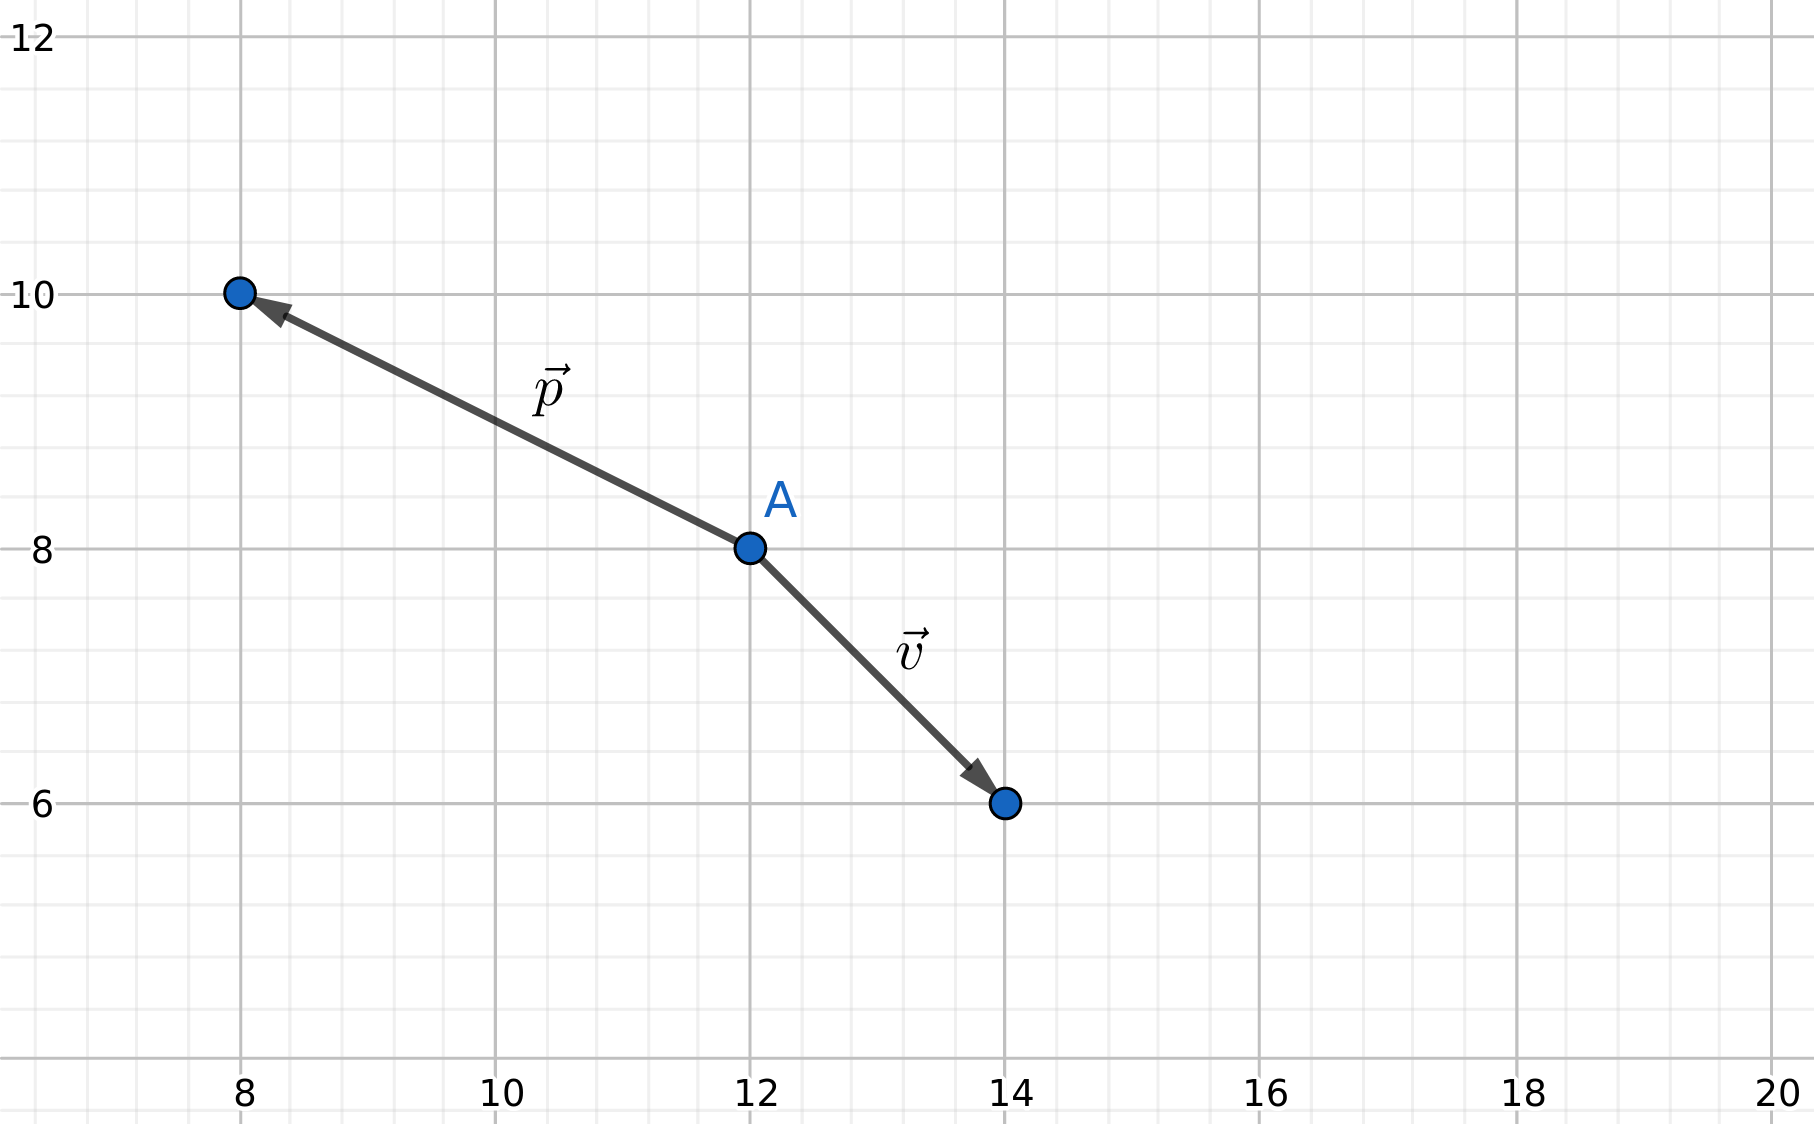
\includegraphics[width=.9\linewidth]{assets/vec2.png}
%\small{Incluir vetor p aqui}
\end{minipage}

% 2º linha
\begin{minipage}{0.48\textwidth}
\centering
\caption{Vetor $\vec g$ de o $gBest$}
\label{fig:vetor-g}
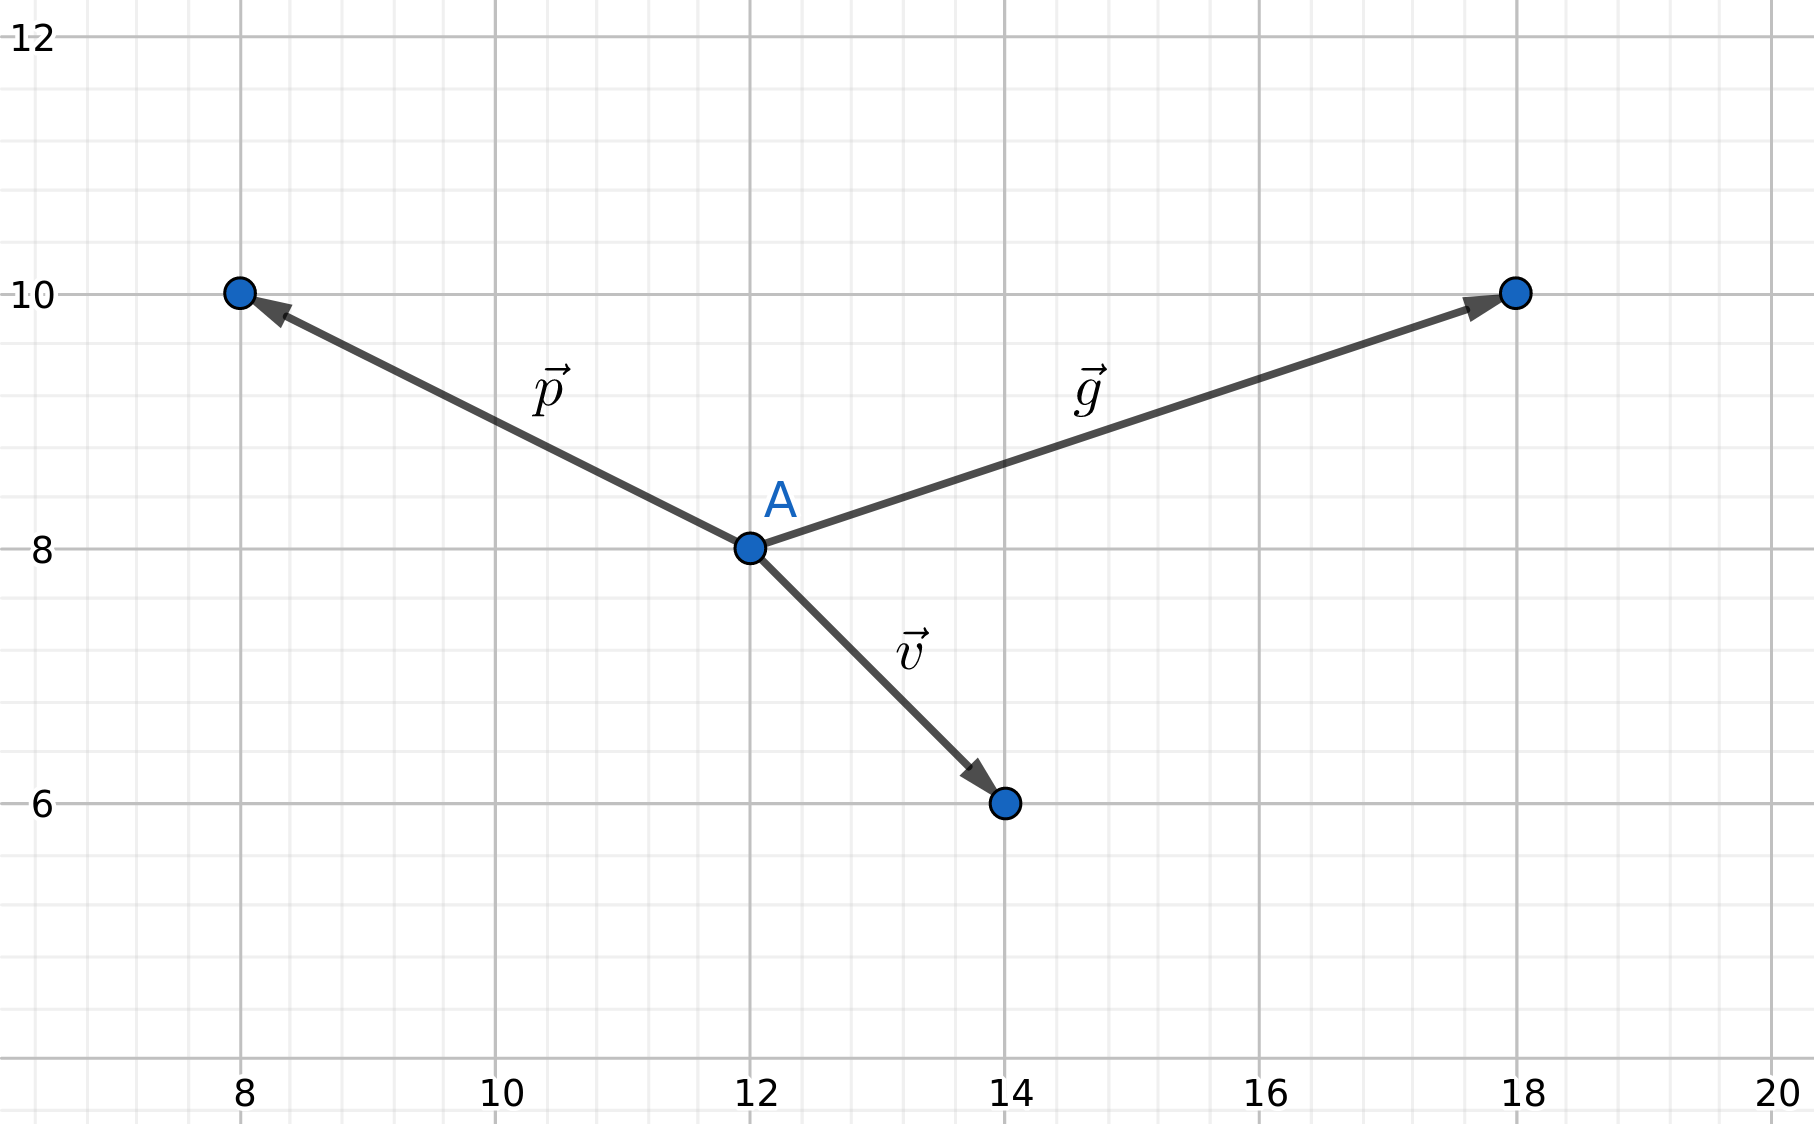
\includegraphics[width=.9\linewidth]{assets/vec3.png}
%\small{Incluir vetor g aqui}
\end{minipage}
\begin{minipage}{0.48\textwidth}
\centering
\caption{Vetor $\vec r$ de movimento final}
\label{fig:vetor-r}
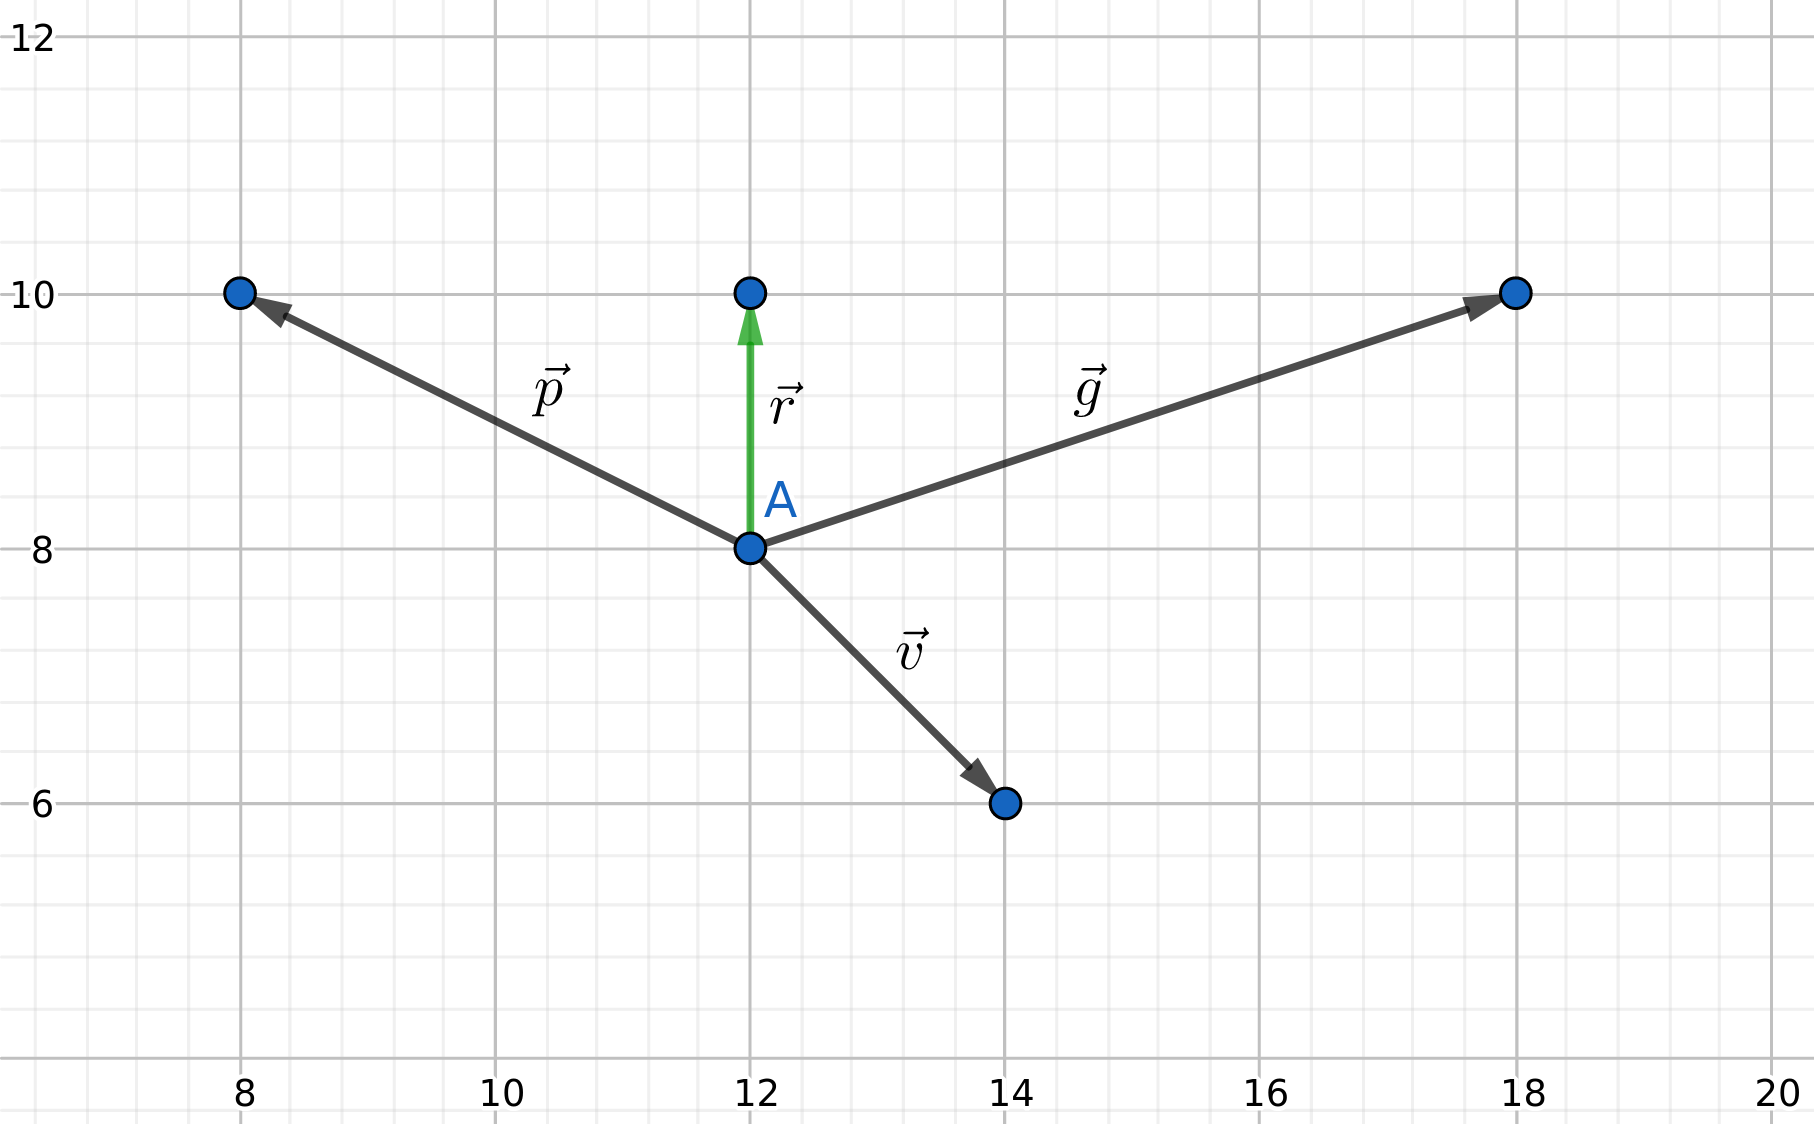
\includegraphics[width=.9\linewidth]{assets/vec4.png}
%\small{Incluir vetor w aqui}
\end{minipage}

\end{minipage}
\end{figure}

\noindent A nova posição da partícula é dada pela 
\hyperref[eq:movimentacao-vec]{Equação \ref{eq:movimentacao-vec}}
.
%
\begin{equation} 
    \label{eq:movimentacao-vec}
    \vec r = ((\vec g + \vec p) / 2) + \vec v
\end{equation}

\noindent Então temos o vetor $\vec r$ resultante, então a nova posição da partícula é $[12,10]$.

No código Python essa implementação é feita de maneira levemente diferente por características da linguagem. Para realizar os cálculos vetoriais foi utilizado a biblioteca \textit{Numpy}.\\
\indent Para isso primeiro é calculado um vetor médio entre $pBest$ e $gBest$, e o vetor $\vec w$ representando a inércia.\\
\indent Então a posição atual da partícula é deduzido do valor médio entre $pBest$ e $gBest$, isso é feito para que calcular o vetor como se a posição atual da partícula fosse o ponto $[0,0]$ do mapa.\\
Então somado com o vetor de inércia divido por um valor de significância para a inércia (Definido pelos parâmetros de configuração do algoritmo).\\
%
\indent No \hyperref[alg:mov-part]{Pseudocódigo \ref{alg:mov-part}} é possível ver a representação dessa função de cálculo, e a implementação desse método está disponível no apêndice x.
%% TODO - apêndice
\begin{algorithm}
    \caption{Pseudocódigo de movimentação de particula}\label{alg:mov-part}
\begin{algorithmic}
\State vetor de inercia $\gets$ (posicao inicial $*$ velocidade)
\State melhor media $\gets$ ($pBest$ + $gBest$) / 2
\State vetor final $\gets$ (melhor media + posição inicial) / 2
\end{algorithmic}
\end{algorithm}
%% Fim do [Movimentação Vetorial] %%
%% Fim do [Movimentação] %%
%% Fim do [Partícula] %%
%% 2 ::: Desenvolvimento
%% 2.2 ::: Arquitetura
%% 2.2.4
\subsection{População}
Pelo algoritmo PSO ser um algoritmo baseado em inteligência populacional, ele é muito influenciado pela geração da população inicial, mesmo nos algoritmos com variações aonde existem mutações e consequentemente evolução dos indivíduos da população, as características como inercia, velocidade, direção e posição desses indivíduos da população inicial são de grande importância.\\
%
%
\indent Os parâmetros como o tamanho da população são definidos nas configurações de hiper parâmetros do algoritmo.
%
Já as funções utilizadas na geração dos indivíduos iniciais utilizam alguns valores aleatórios que seguem um padrão de distribuição uniforme. Os atributos que utilizam valores aleatórios são:
\begin{itemize}
    \item A velocidade, que é dada por um valor aleatório entre $0.1$ e $0.2$.
    \item A posição inicial da partícula, que é dada por dois números aleatórios entre $1$ e o limite do espaço de soluções $- 1$.
    \item A última posição da partícula, que é obtida através de um numero inteiro aleatório entre $1$ e $-1$ diferente de zero.
\end{itemize}
%
%
\indent Assim, como valores iniciais seguindo uma distribuição uniforme é observado uma geração de população inicial bem distribuída, dificultando o acontecimento de convergência prematura.\\
%
%
Sendo assim, todas as variações do algoritmo PSO implementadas nesse trabalho utilizam a mesma função geradora de população inicial, cujo a implementação está no 
\hyperref[apd:fun-gen-init-pop]{Apêndice \ref{apd:fun-gen-init-pop}}
%%% 
\noindent Garantindo assim um ponto de comparação mais justo entre os algoritmos.
%% 2 ::: Desenvolvimento
%% 2.2 ::: Arquitetura
%% 2.2.5
\subsection{Algoritmos}
%%
A execução dos algoritmos é chamada pela classe principal de modelagem do problema, responsavel por fazer a execução e controle dos dados de analise.\\
%
Na classe do PSO estão as funções da condição de parada, movimento e \textit{evaluete} do \textit{fitness} da particula. A implementação esta disponivel no apendice x.\\ %todo apendice
%
%
Como criterio de parada para o algoritmo foi utilizado o fator de atualização do $gBest$. Quando a ultima atualização do $gBest$ for a mais rodadas do que metade da quantidade de particulas, o algoritmo termina e o resultado é o $gBest$ atual.\\
%%
\indent O que diferencia as abordagens analisadas nesse trabalho são as heuristicas de movimentação das particulas.\\
A movimentação basica de uma particula do PSO é definido pela
\hyperref[eq:movimentacao-particula]{Equação \ref{eq:movimentacao-particula}}
.
%
\begin{equation} 
    \label{eq:movimentacao-particula}
    \vec v_1(t+1)= \vec v_i(t) + a_1 r_1 (pBest - \vec x_i(t)) + a_2 r_2 (gBest - \vec x_i(t))
\end{equation}
%
Como foi observado nos testes a variavel aleatoria é importande para que as particulas não entrem em um estado de equilibrio e parem de se movimentar. Com a introdução de elementos aleatorio a movimentaçãos se torna mais caotica e evita o fim prematuro do algoritmo.

Esse impacto na movimentação inspirou uma abordagem que considera o nivel de atualizações de $gBest$ e assim adiciona mais um fator aleatorio no calculo. como é representado no 
\hyperref[alg:mov-dinamic]{Pseudocódigo \ref{alg:mov-dinamic}}.
\begin{algorithm}
    \caption{Pseudocódigo de movimentação com componente dinamico}\label{alg:mov-dinamic}
\begin{algorithmic}

\State vetor de inercia $\gets$ (posicao inicial $*$ velocidade)
\State melhor media $\gets$ (($pBest$ + $gBest$) / 2)
\State vetor final $\gets$ ((melhor media + posição inicial) / 2)

\If{trocas de $gBest$ é menor que (tamanho da populacao / $10$)}
    \State vetor final $\gets$ vetor de movimento $+$ $0.1$ $*$ (inercia$*$random($0.1$, $0.9$) )
\Else
    \State vetor final $\gets$ vetor de movimento $+$ $0.1$ $*$ random($0.1$, $0.9$) 
\EndIf    
\end{algorithmic}
\end{algorithm}

%% Fim do [Algoritmos] %%
%% Fim do [Arquitetura] %%
%% 2 ::: Desenvolvimento
%% 2.3
\section{Execuções}
Foram utilizados como parâmetros de configuração:
\begin{itemize}
    \item \code{population\_size} Quantidade de particulas
    \item \code{coeficente\_populacional}: Coeficiente entre a quantidade de particulas e o tamanho do espaço de soluções
\end{itemize}
%
O tamanho do espaço de soluções é calculado pela raiz do arrendamento para baixo do tamanho da população elevado ao coeficiente populacional, representado pela equação 
\hyperref[eq:space-size]{Equação \ref{eq:space-size}}, 
essa equação é necessaria pois para gerar um espaco de soluções $n \times n$ pois para isso o numero precisa ser uma raiz quadrada perfeita.
%
\begin{equation} 
    \label{eq:space-size}
    space\_size = \lfloor \sqrt{\lfloor n^c \rceil} \rceil
\end{equation}
%
Para essa analise foram usados os valores de \code{population\_size = 30} e o 3 valores diferentes de coeficente populacional que são:
\begin{itemize}
    \item \code{coeficente\_populacional = $3$}: Gera um mapa de $50 \times 50$
    \item \code{coeficente\_populacional = $5$}: Gera um mapa de $70 \times 70$
    \item \code{coeficente\_populacional = $2.645$}: Gera um mapa de $90 \times 90$
\end{itemize}

Foram gerados 20 espaços de solução diferentes para cada cada um dos 3 coeficentes e cada um dos 4 cenarios de problema diferentes que estão no 
\hyperref[apd:problem-instances]{Apendice \ref{apd:problem-instances}}, totalizando assim $240$ espaços de soluções diferentes.\\
%
Pela natureza variável do ambiente em nuvem e por se tratar de um algoritmo que utiliza fatores aleatorios, a execução de cada uma das 2 abordagens foi repetida 20 vezes para assim obter uma média mais precisa das soluções de cada algoritmo.\\
%
Como foi descrito anteriormente, de modo a assegurar uma análise posterior mais detalhada, os dados gerados pelos algoritmos foram salvos em aquivo binario.\\
Os dados salvos são:
\begin{itemize}
    \item População inicial.
    \item Espaço de soluções.
    \item Números de rodadas do algoritmo.
    \item Histórico da variável $gBest$.
    \item Histórico da posição das partículas.
    \item Soluções encontradas.
\end{itemize}
%% 2 ::: Desenvolvimento
\section{Resultados}
Para avaliar as execuções dos algoritmos foram estabelecidos os seguintes criterios de analise:
A partir das médias estatísticas das execuções, são utilizados como critérios de avaliação do algoritmo:
\begin{itemize}
\item Makespan final das soluções
\end{itemize}

\noindent E são parâmetros de análise:
\begin{itemize}
\item Taxa de mudança da variável $gBest$ ao longo da execução.
\item Quantidade de rodadas necessárias para atingir o critério de parada.
\item Taxa de mudanças de $pBest$ por rodada.
\item Histórico de movimentação das partículas.
\end{itemize}

(Dados a completar...)
%
%% Fim do [Resultados] %%
